\documentclass[final,hyperref={pdfpagelabels=false}]{beamer}
\usepackage{grffile}
\mode<presentation>{\usetheme{PosterLogProb}}
\usepackage[english]{babel}
\usepackage[latin1]{inputenc}
\usepackage{amsmath,amsthm, amssymb, latexsym}
\usepackage{epsfig}
\usepackage{listings}
\usepackage{lstlinebgrd}

\usepackage[orientation=portrait,size=a0,scale=1.4,debug]{beamerposter}
\providecommand\thispdfpagelabel[1]{}
\setbeamertemplate{bibliography entry title}{\color{black}}
\setbeamertemplate{bibliography entry location}{}
\setbeamertemplate{bibliography entry note}{}

\usepackage{array,booktabs,tabularx}
\newcolumntype{Z}{>{\centering\arraybackslash}X} % centered tabularx columns
\newcommand{\pphantom}{\textcolor{ta3aluminium}} % phantom introduces a vertical space in p formatted table columns??!!

\listfiles

\usepackage{amsthm}
%%%%%%%%%%%%%%%%%%%%%%%%%%%%%%%%%%%%%%%%%%%%%%%%%%%%%%%%%%%%%%%%%%%%%%%%%%%%%%%%%%%%%%


 \title{\huge\bfseries\hspace*{-1em} Empurrando Juntos: \\A platform for social participation}
\date{}
\author{\large Tallys Martins
\and Dylan Guedes
\and Luan Guimarães \\
\and Ricardo Poppi
\and Henrique Parra
\and Paulo Meirelles
}
\institute[UNB/CD]{University of Brasília and Cidade Democrática NGO, Brazil}

\newlength{\columnheight}
\setlength{\columnheight}{105cm}


\begin{document}
\setbeamertemplate{caption}{\raggedright\insertcaption\par}
\begin{frame}
  \begin{columns}
    % ---------------------------------------------------------%
    % Set up a column
    \begin{column}{.49\textwidth}
      \begin{beamercolorbox}[center,wd=\textwidth]{postercolumn}
        \begin{minipage}[T]{.95\textwidth}
          \parbox[t][\columnheight]{\textwidth}{

\begin{block}{Facing the bubbles}
  \begin{itemize}
    \item Social media recommendation algorithms are black boxes
    
    \item Engines and systems are specialized in analyzing our profiles. We only receive
    content about what we like, what we follow and what our friends see.

    \item People are stuck in a phenomenon that we call ``bubbles of opinion``

    \item The bubbles caused by this algorithms unbalance the dialog and minorities
    are despised.
  \end{itemize}
\end{block}

\begin{block}{Polis}
  \begin{itemize}
    \item Polis is a web based platform for online debates that uses A.I. to
    show the different opinion groups in a discussion.

    \item Allow people to create online conversations to debate about any subject,
    anonymous or not, and uses a different approach to build the dialog between users.

    \item Using a concept that we call ``crowdsource participation``, people can
    give their opinion by simple clicking in ``agree``, ``disagree`` or ``skip``
    in other's comments. Participation gets easier in a one click effort.

    \item The system applies clustering algorithms to identify the different groups
    of opinion based on the reactions of the participants in the comments.

    \item The majority and minority consensus is showed in a graph, and can be
    displayed in the global scope considering all the participants or in each group
    scope.
  \end{itemize}

  \begin{figure}
    \begin{center}
      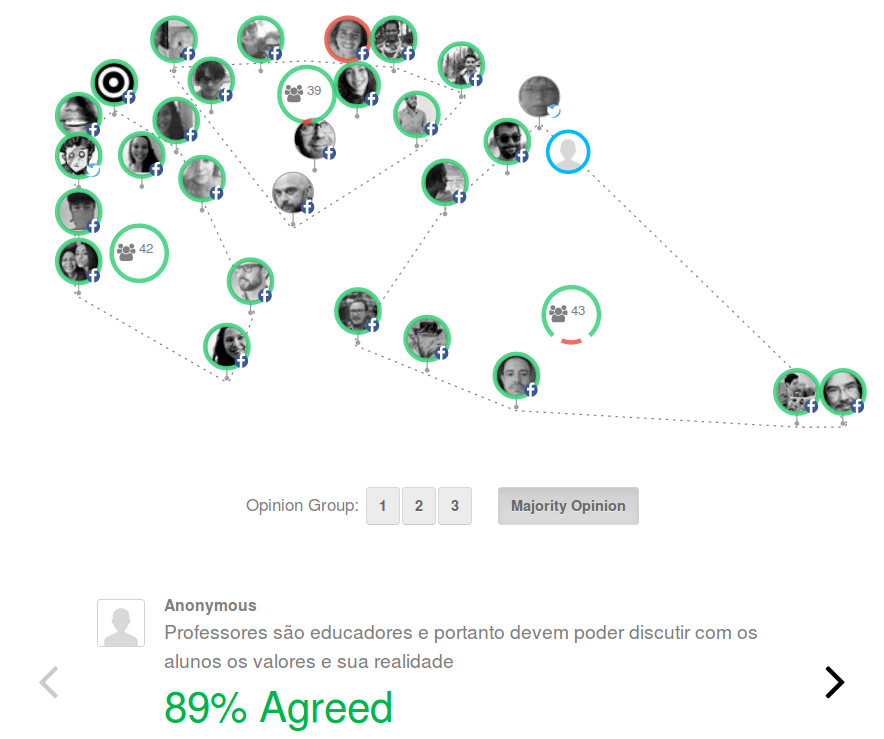
\includegraphics[scale=1.1]{../images/polis3.png}
      \caption{Groups of opinion formed by Polis}
      \label{fig:group-clusters}
    \end{center}
  \end{figure}
\end{block}

\begin{block}{What is Empujando Juntos}

  \begin{itemize}
    \item A Free Open Source Software for social participation that aims to
    increase communication between majority and minority, blowing bubbles of
    opinion.

    \item An platform built on top of Polis that offers new features
    with gamification concepts.
    
    \item A tool that allows activists and non extremist people to engage regular
    people in online discussions.
  \end{itemize}
\end{block}

\begin{block}{Why Empurrando Juntos?}
  \begin{itemize}
    \item E.J. goes beyond Polis by adding new features that offers more interaction
    to the discussions.

    \item Uses gamification concepts based on the profiles of the participants as
    a mean to bring diversity to online discussions.
  \end{itemize}
\end{block}


%-------------------------------------------------------------------------------
}
\end{minipage}
\end{beamercolorbox}
\end{column}
% ---------------------------------------------------------%
% end the column

% ---------------------------------------------------------%
% Set up a column
\begin{column}{.49\textwidth}
  \begin{beamercolorbox}[center,wd=\textwidth]{postercolumn}
    \begin{minipage}[T]{.95\textwidth} % tweaks the width, makes a new \textwidth
      \parbox[t][\columnheight]{\textwidth}{ % must be some better way to set the the height, width and textwidth simultaneously

\begin{block}{Empujando Juntos Features}
  \begin{itemize}
    \item Uses Polis engine to obtain the groups of opinion.

    \item Provides a resource that we called ``the Push``. People in ownership of
    this ability (gamification) can access special features in the platform.

    \item The ``Push`` is given to special actors in the groups formed by Polis.
    Three profiles are considered, the activist, the bridge and the consultation
    owner.

    \item Monitor Polis conversations created through the App
    to identify activists and bridge participants and give them the ``Push``
    power.

    \begin{figure}
      \begin{center}
        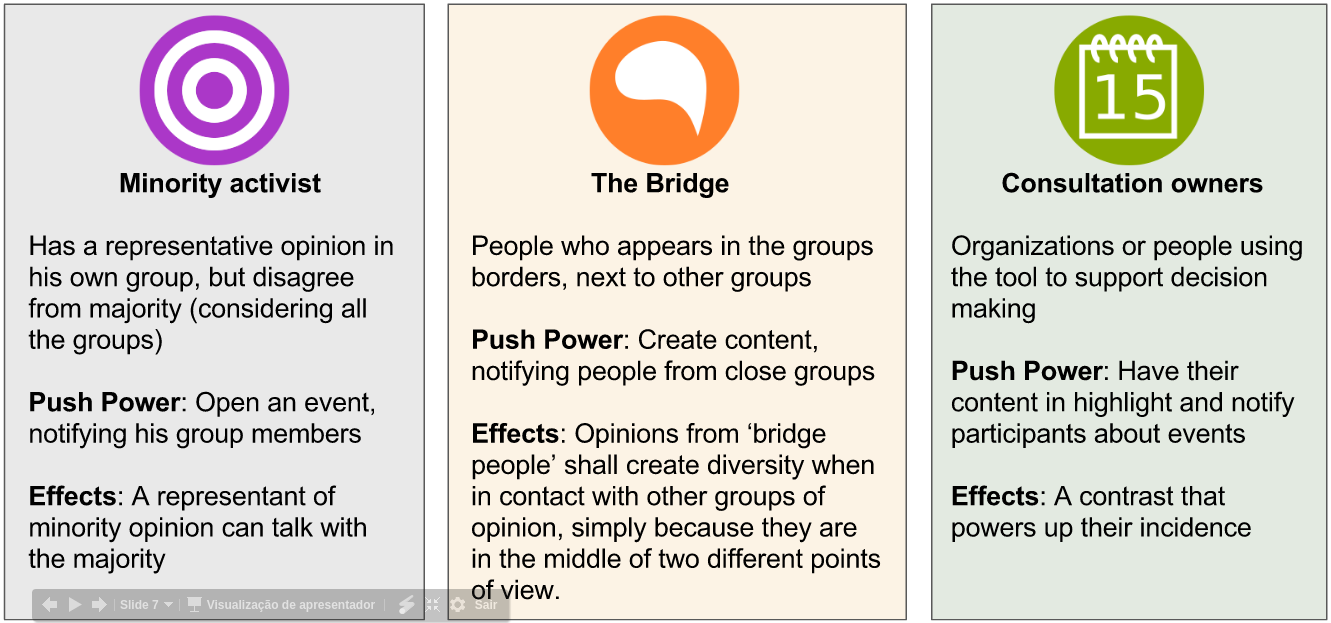
\includegraphics[scale=1.4]{../images/userprofiles.png}
        \caption{Profiles identified by Empurrando Juntos}
        \label{fig:user-profiles}
      \end{center}
    \end{figure}
  \end{itemize}
\end{block}

\begin{block}{System Architecture}
	\begin{itemize}
    \item Front-end application, written in React Native
    and a NodeJS server.

    \item The server module is responsible for managing users, ``the Push'', and
    to make the interface with Polis API
  \end{itemize}

  \begin{figure}
    \begin{center}
      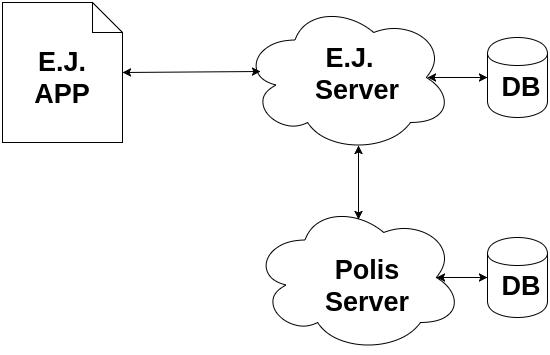
\includegraphics[scale=1.3]{../images/polis4.png}
      \caption{Simplified architecture of the system}
      \label{fig:architecture}
    \end{center}
  \end{figure}
\end{block}

\begin{block}{Integration with Polis}
  \begin{itemize}
    \item Other platforms can register the participation of their users on Polis
    through the xID (external id) parameter in the API.

    \item Polis conversations can be easily embed with javascript snippets.

    \item E.J. calculates the profiles based on the conversation data, but future
    implementations aims to include this features inside the core of the clusters
    math and provide them easier through API endpoints.
  \end{itemize}
\end{block}

\begin{block}{Final Remarks}
  \begin{itemize}
    \item Pushing Together arise as a potential tool to bridge dialog between society and
    the state, making different analyzes about the opinion of the distinct groups
    and also opening new possibilities for the expression of these opinions with ``the
    Push`` resource.

    \item We are now working on a research to evolve the clustering service that
    will fit our application model. Parallelly, our next steps include evolving the
    mobile application using mocked data and validating the user interface.

    \item All our contributions are published in open repositories available at:
      \begin{itemize}
        \item \url{github.com/cidadedemocratica/pushingtogether}
        \item \url{github.com/cidadedemocratica/app_pushingtogether}
      \end{itemize}
  \end{itemize}
\end{block}
      }
        \end{minipage}
      \end{beamercolorbox}
    \end{column}
  \end{columns}
\end{frame}
\end{document}
